\chapter{System Visualization Examples}
\label{app:system_examples}

The examples presented here are screenshots of the \acl{gui} of the responsive system presented in \cref{chap:web-based_responsive_spoken_dialogue_system}. These examples compare the state of the system's representation of the \textipa{[e]} vs.\ \textipa{[E]} feature after processing the same user input but using different parameter values (see \cref{sec:parameters,tab:comp_model_parameters}).
It can be seen, for example, how higher sensitivity (top right) leads to faster -- but somewhat unstable -- convergence process that generally imitates the user's productions.
In contrast, the convergence at the top left is too slow to be representative of the user's production.
The two bottom examples demonstrate how taking a larger number of previous exemplars into account leads to a more smoothed convergence process toward some global mean (bottom right) as opposed to more rapidly changing productions that follow only the last encountered exemplar (bottom left).

\begin{landscape}
	\begin{figure}[H]
		\centering
		\hspace*{-4.7cm}
		\scalebox{1.5}{%
			\begin{minipage}{.45\linewidth}
				\centering
				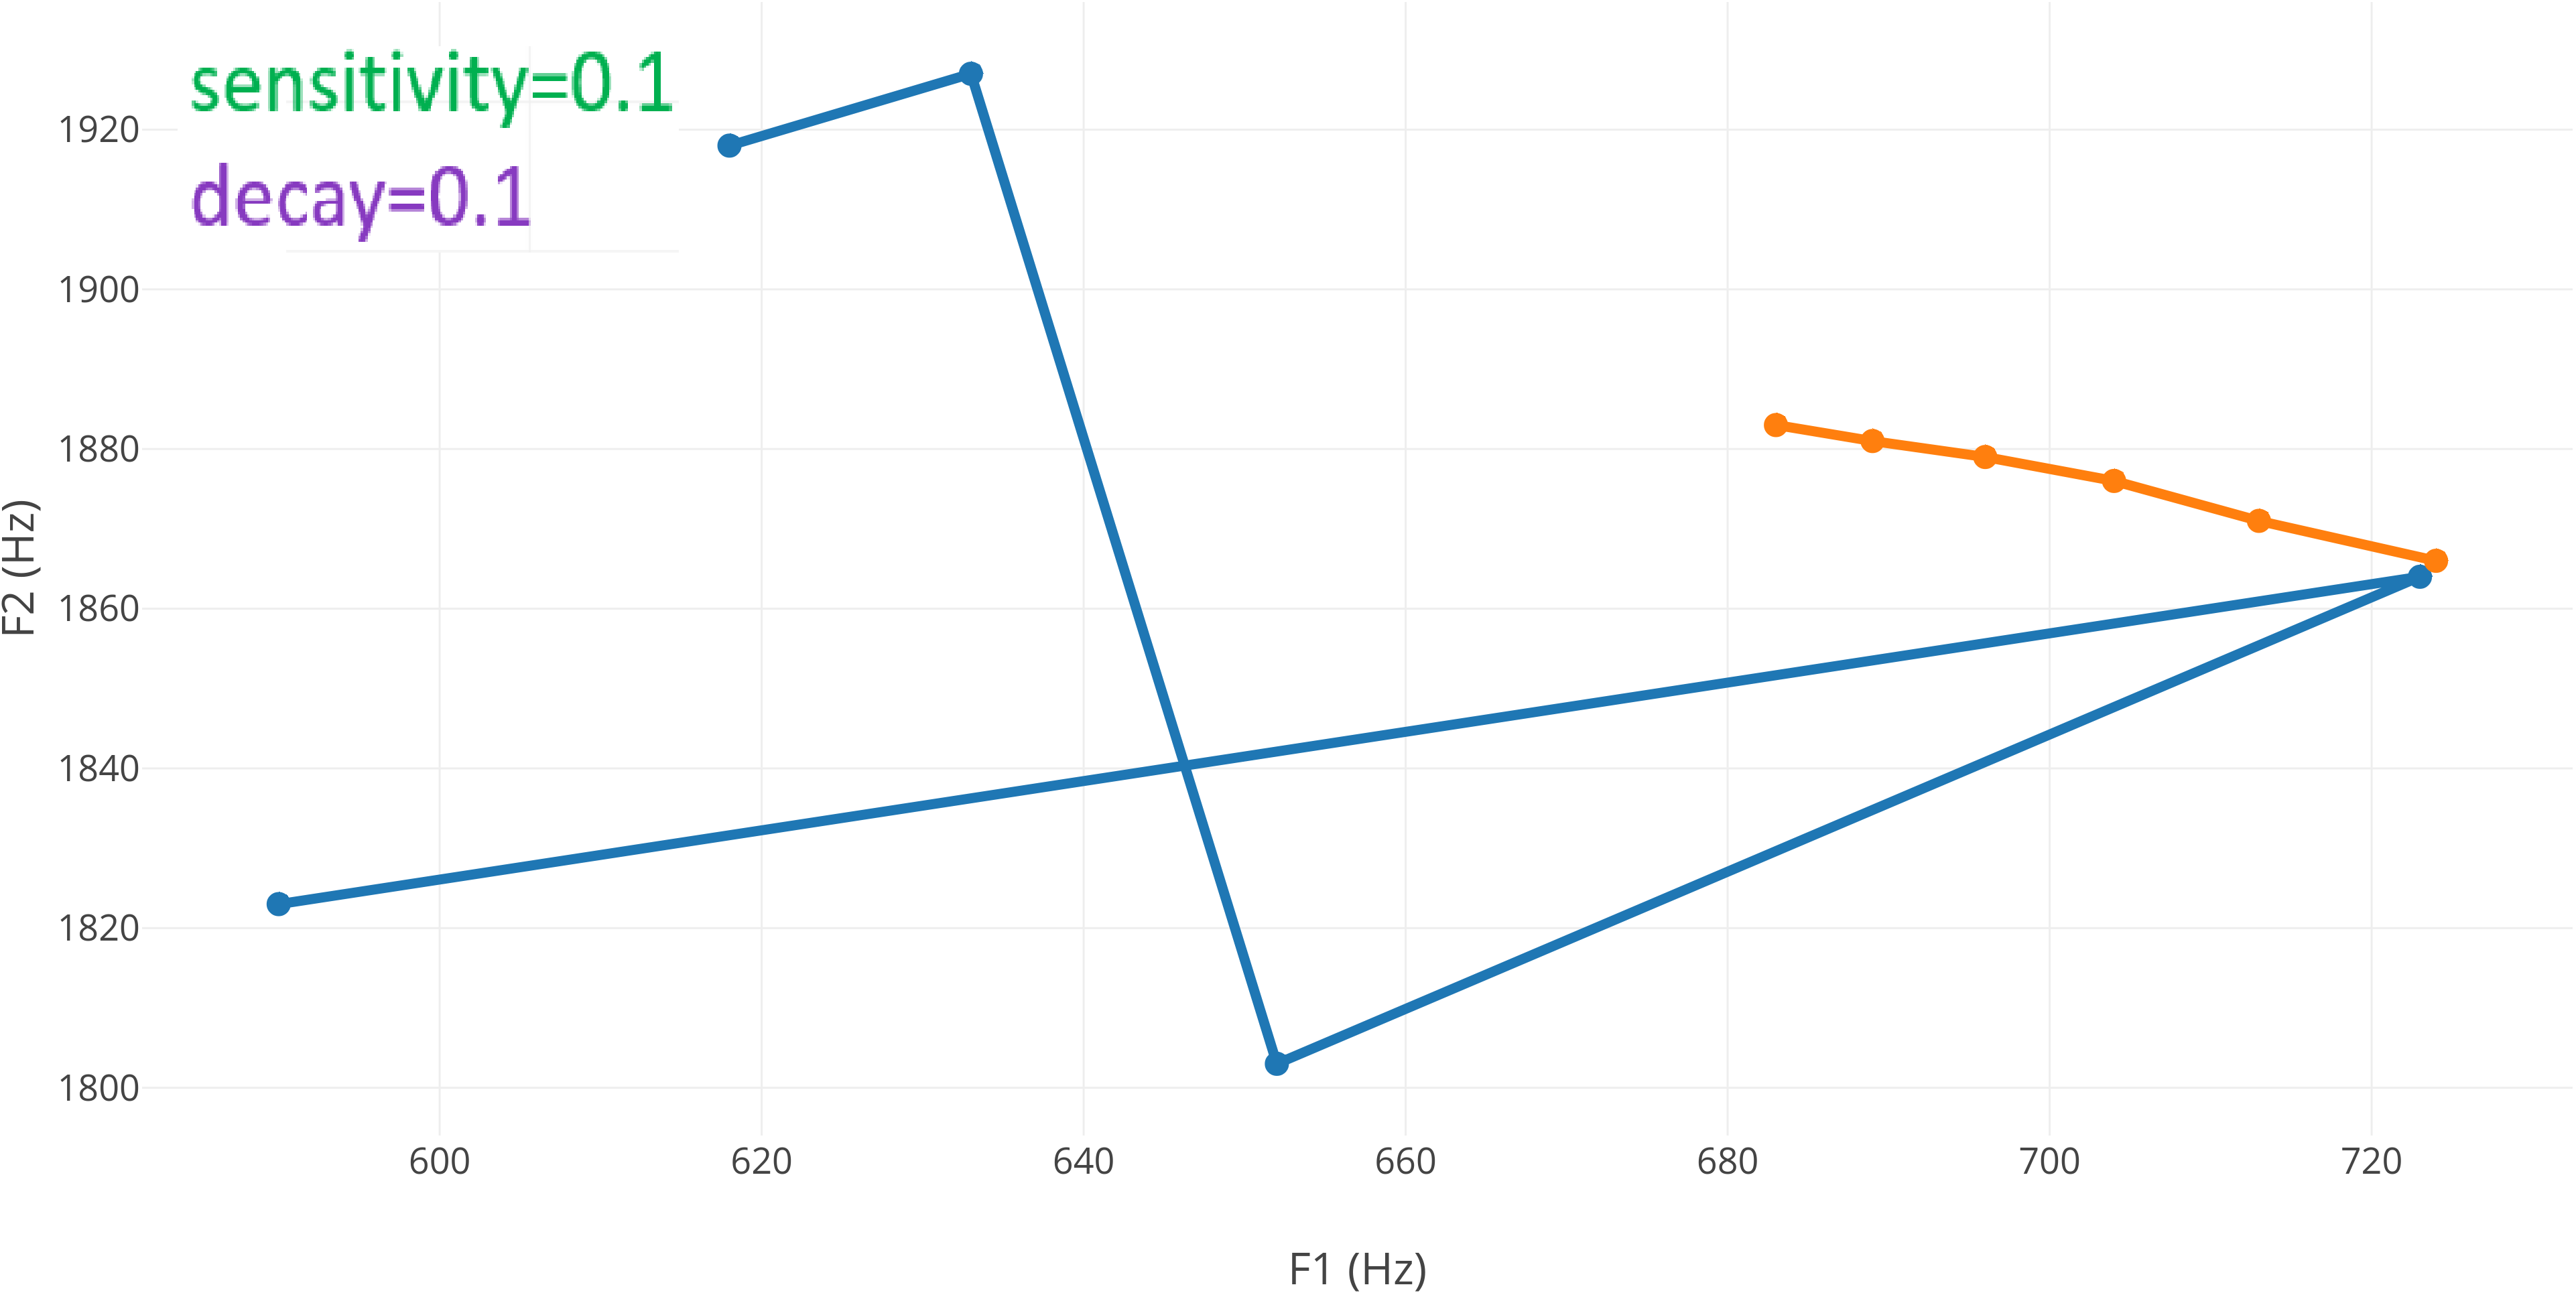
\includegraphics[width=\linewidth]{e_E_01_01_10}
			\end{minipage}%
			\hfill
			\begin{minipage}{.45\linewidth}
				\centering
				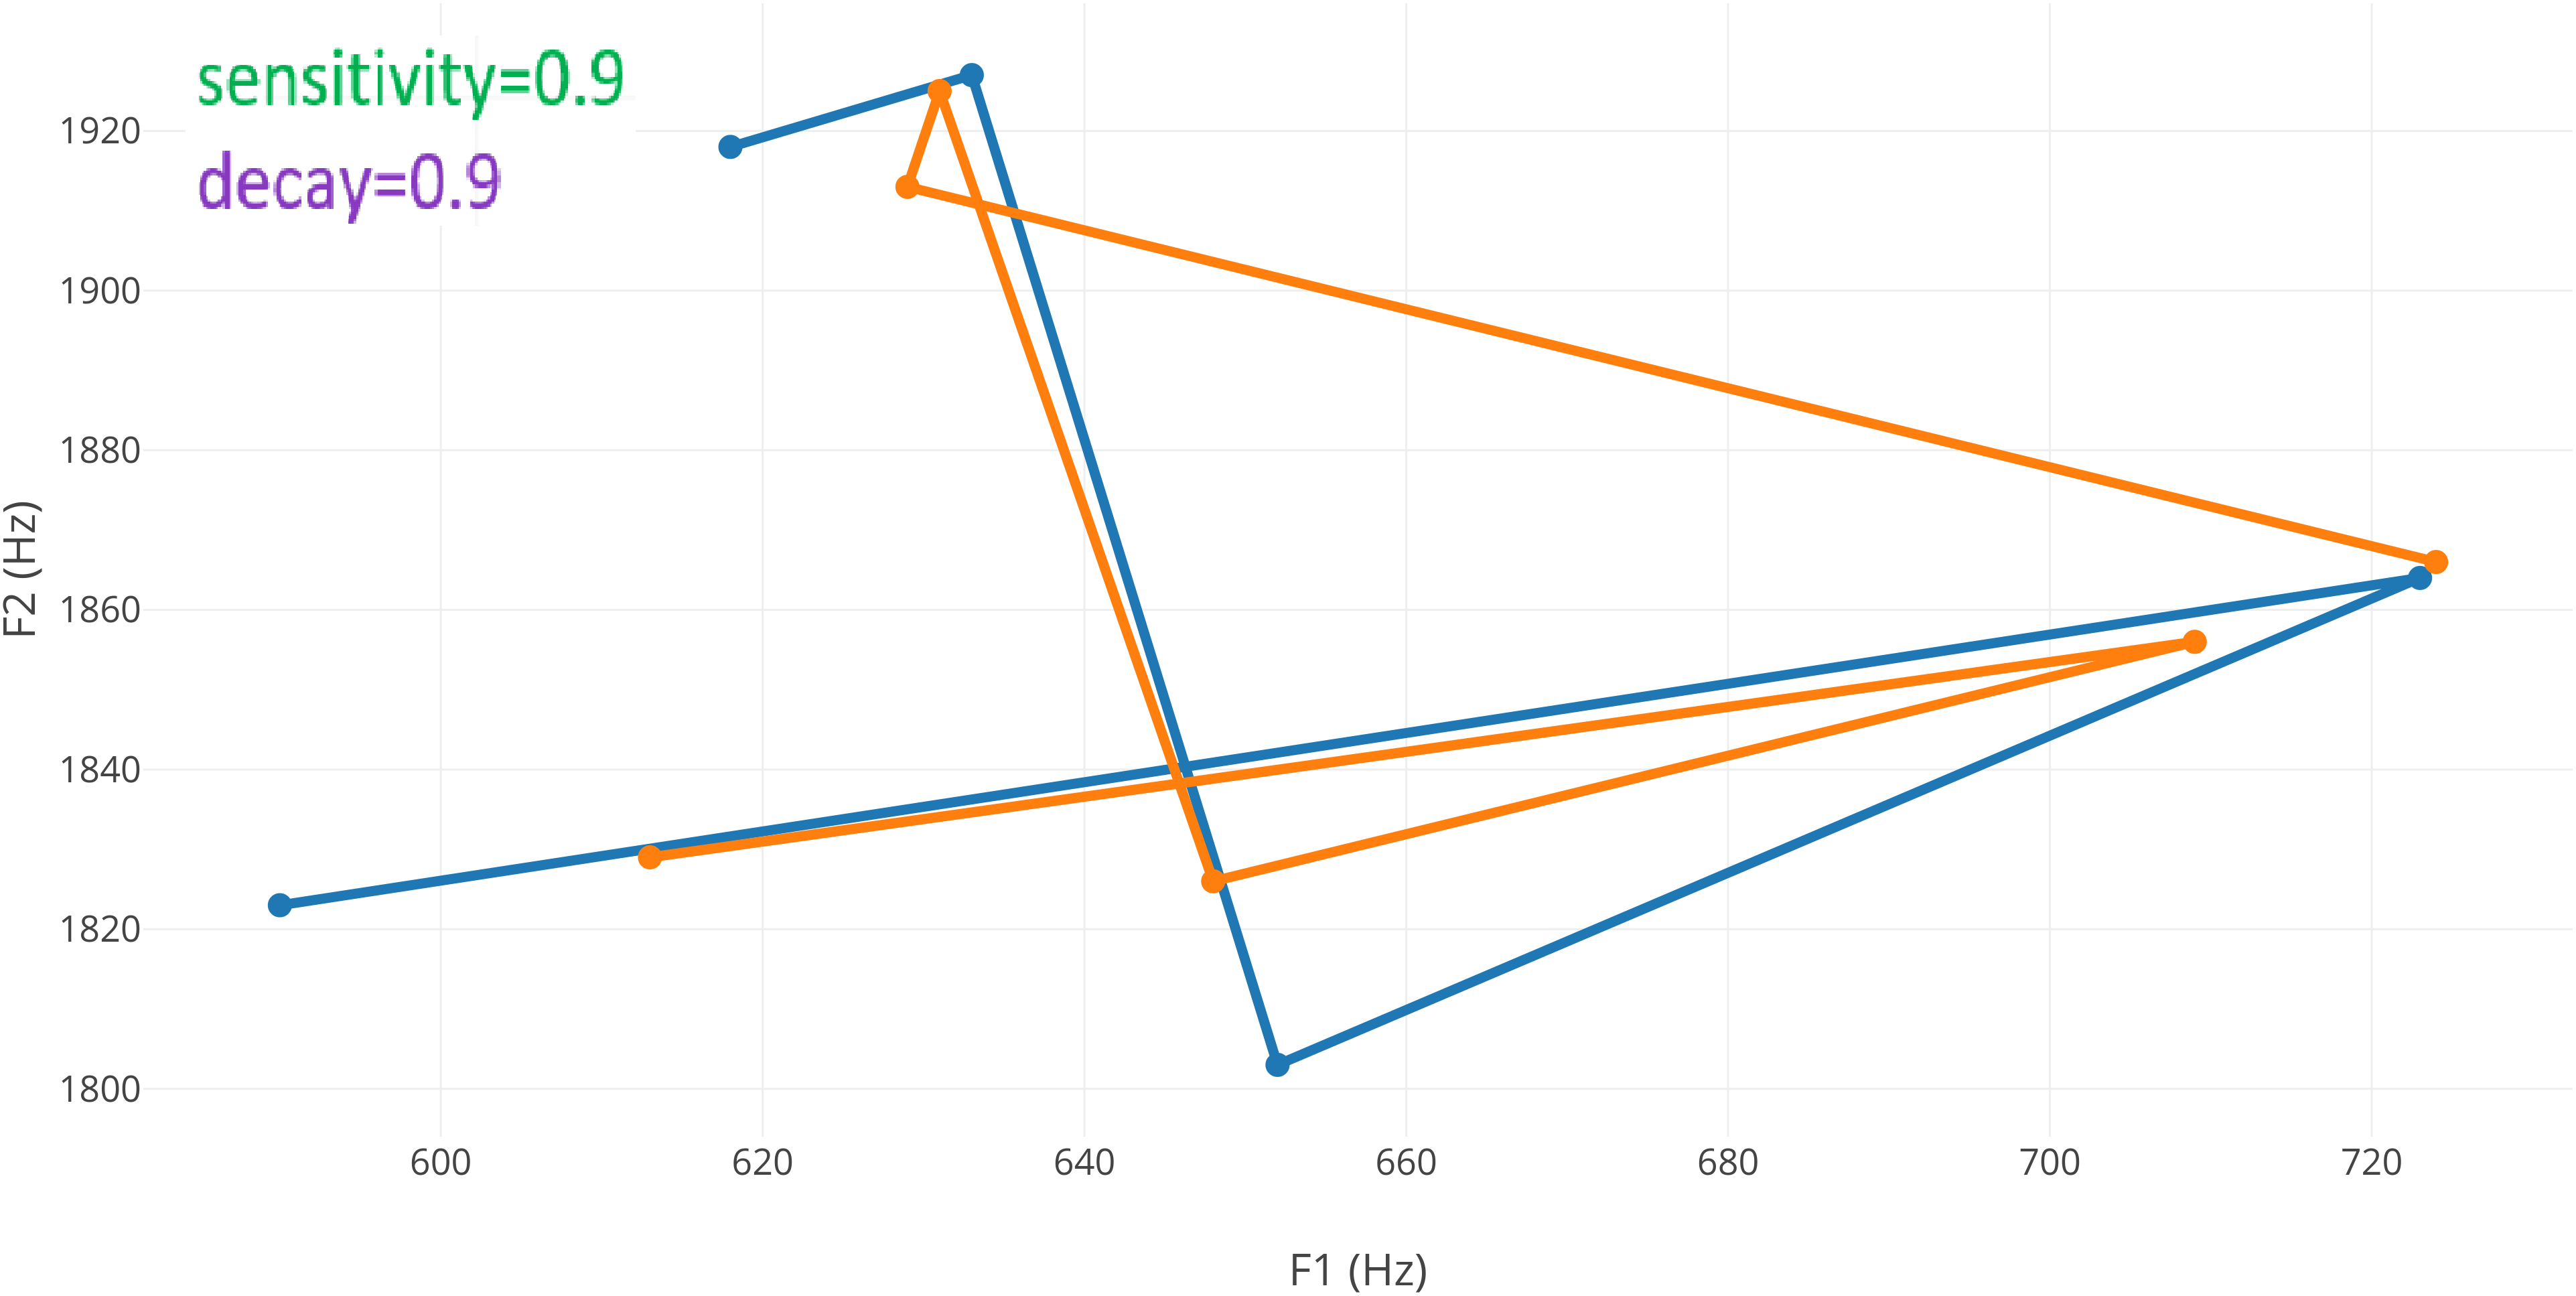
\includegraphics[width=\linewidth]{e_E_09_09_10}
			\end{minipage}
		}
	\end{figure}
	\begin{figure}[H]
		\centering
		\hspace*{-4.7cm}
		\scalebox{1.5}{%
			\begin{minipage}{.45\linewidth}
				\centering
				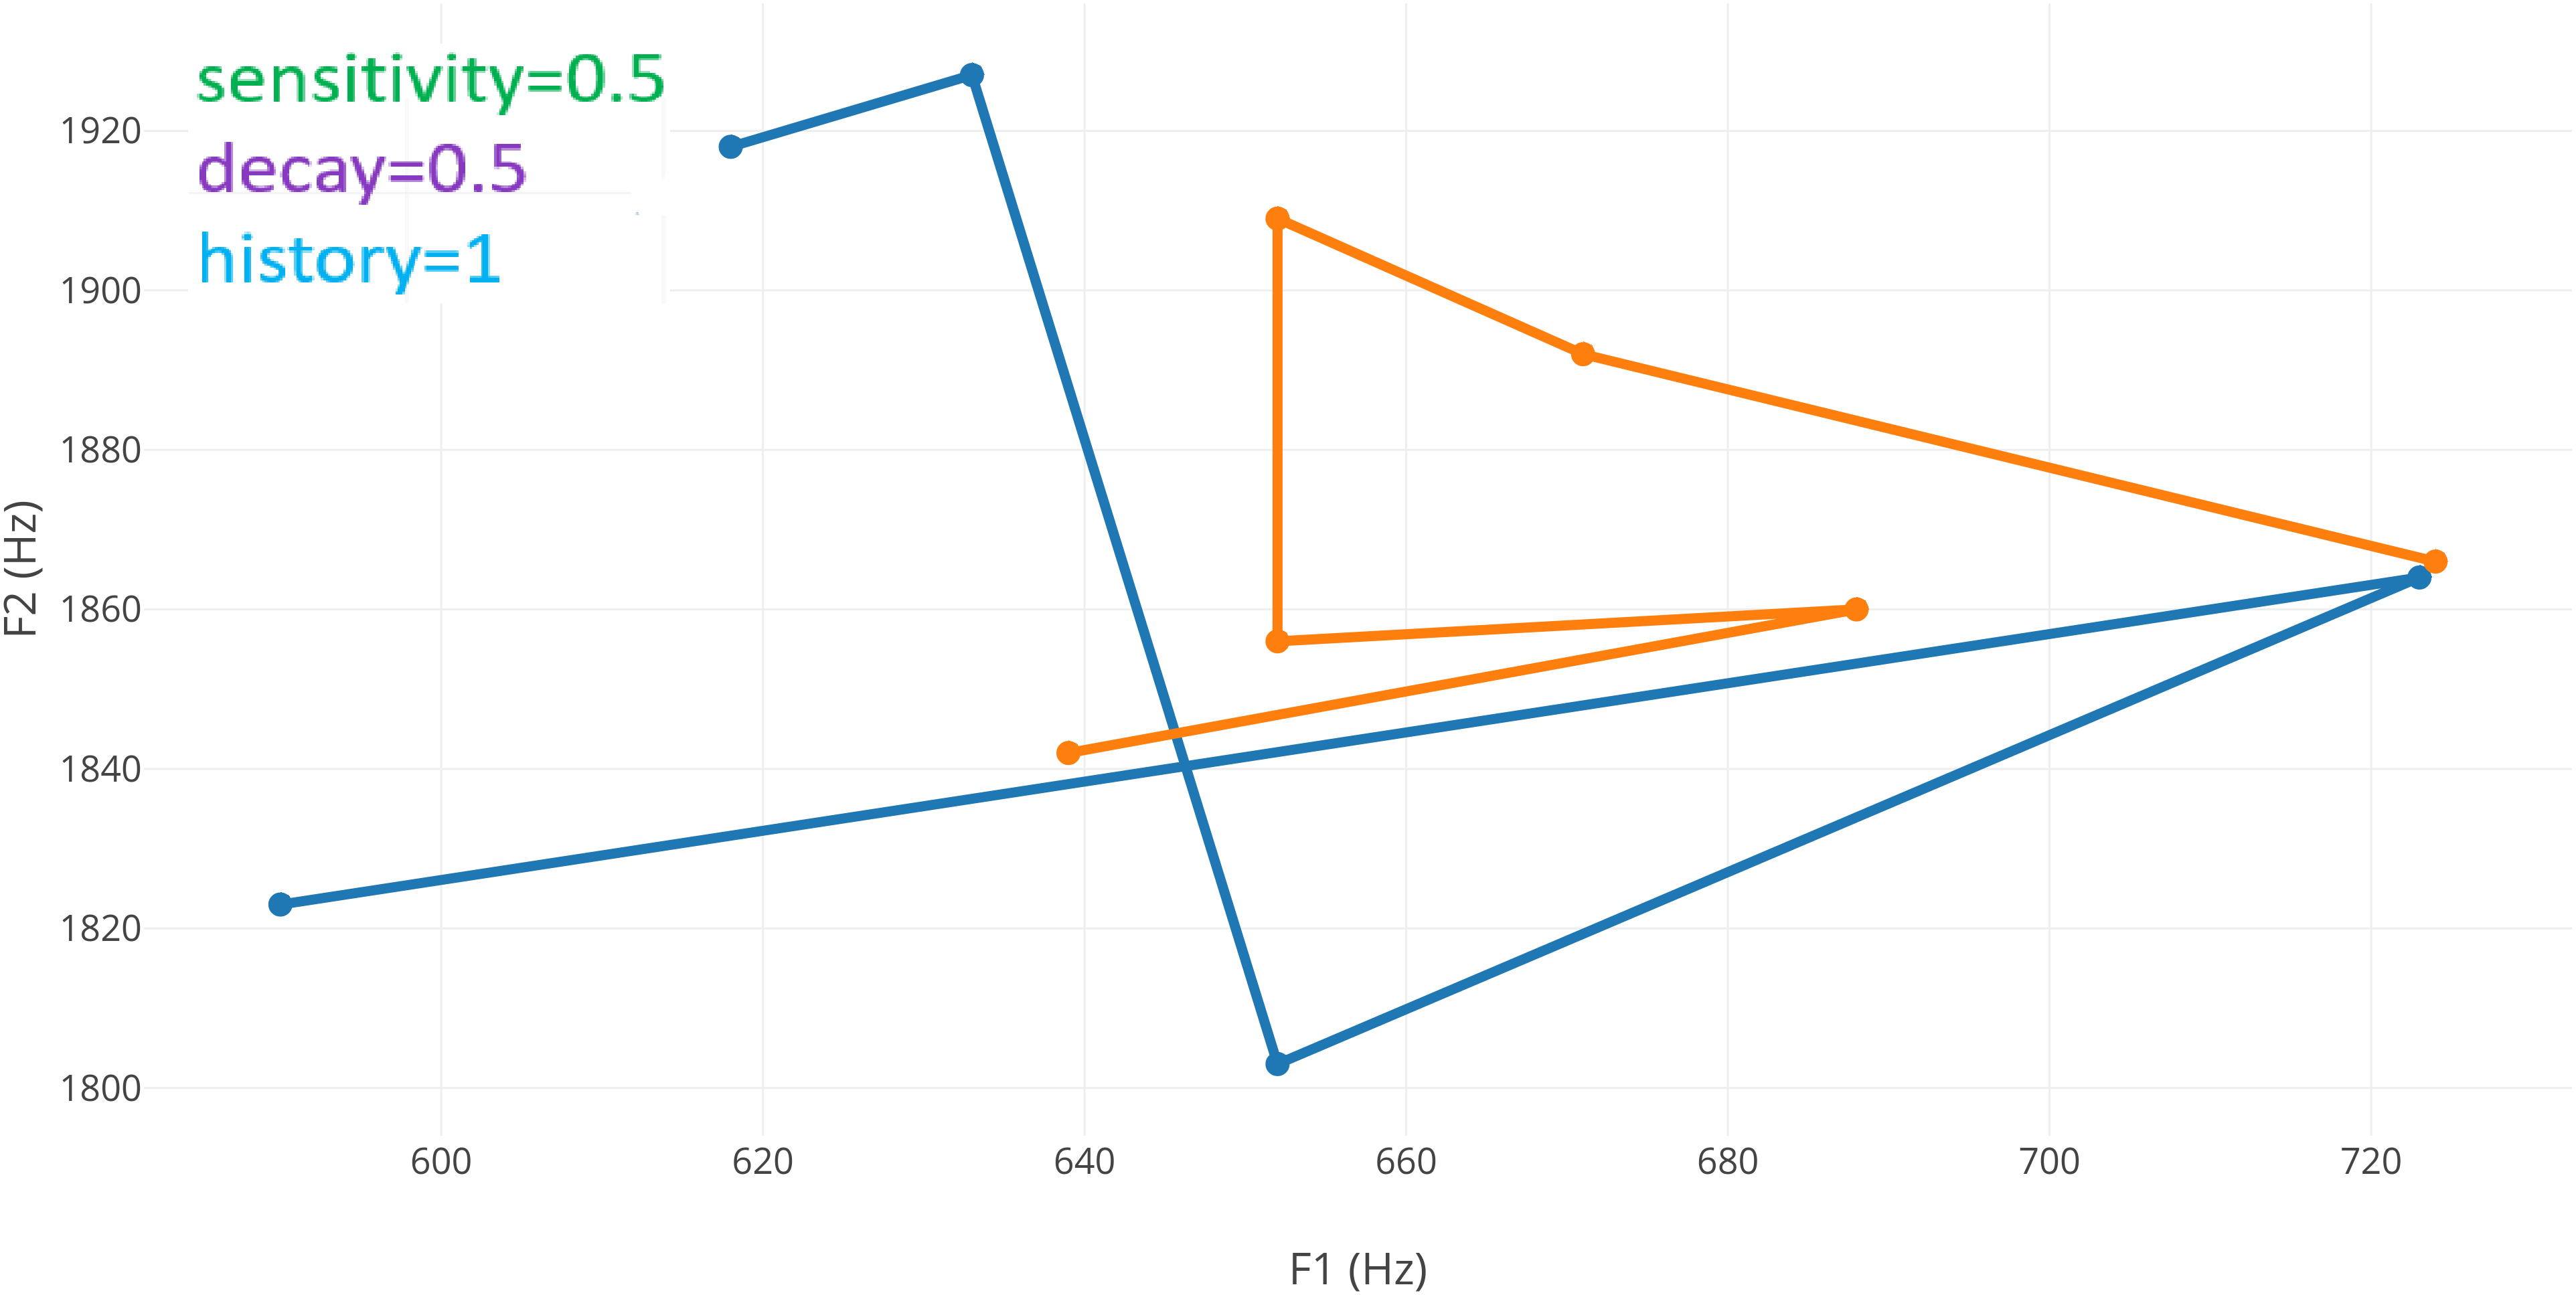
\includegraphics[width=\linewidth]{e_E_05_05_1}
			\end{minipage}%
			\hfill
			\begin{minipage}{.45\linewidth}
				\centering
				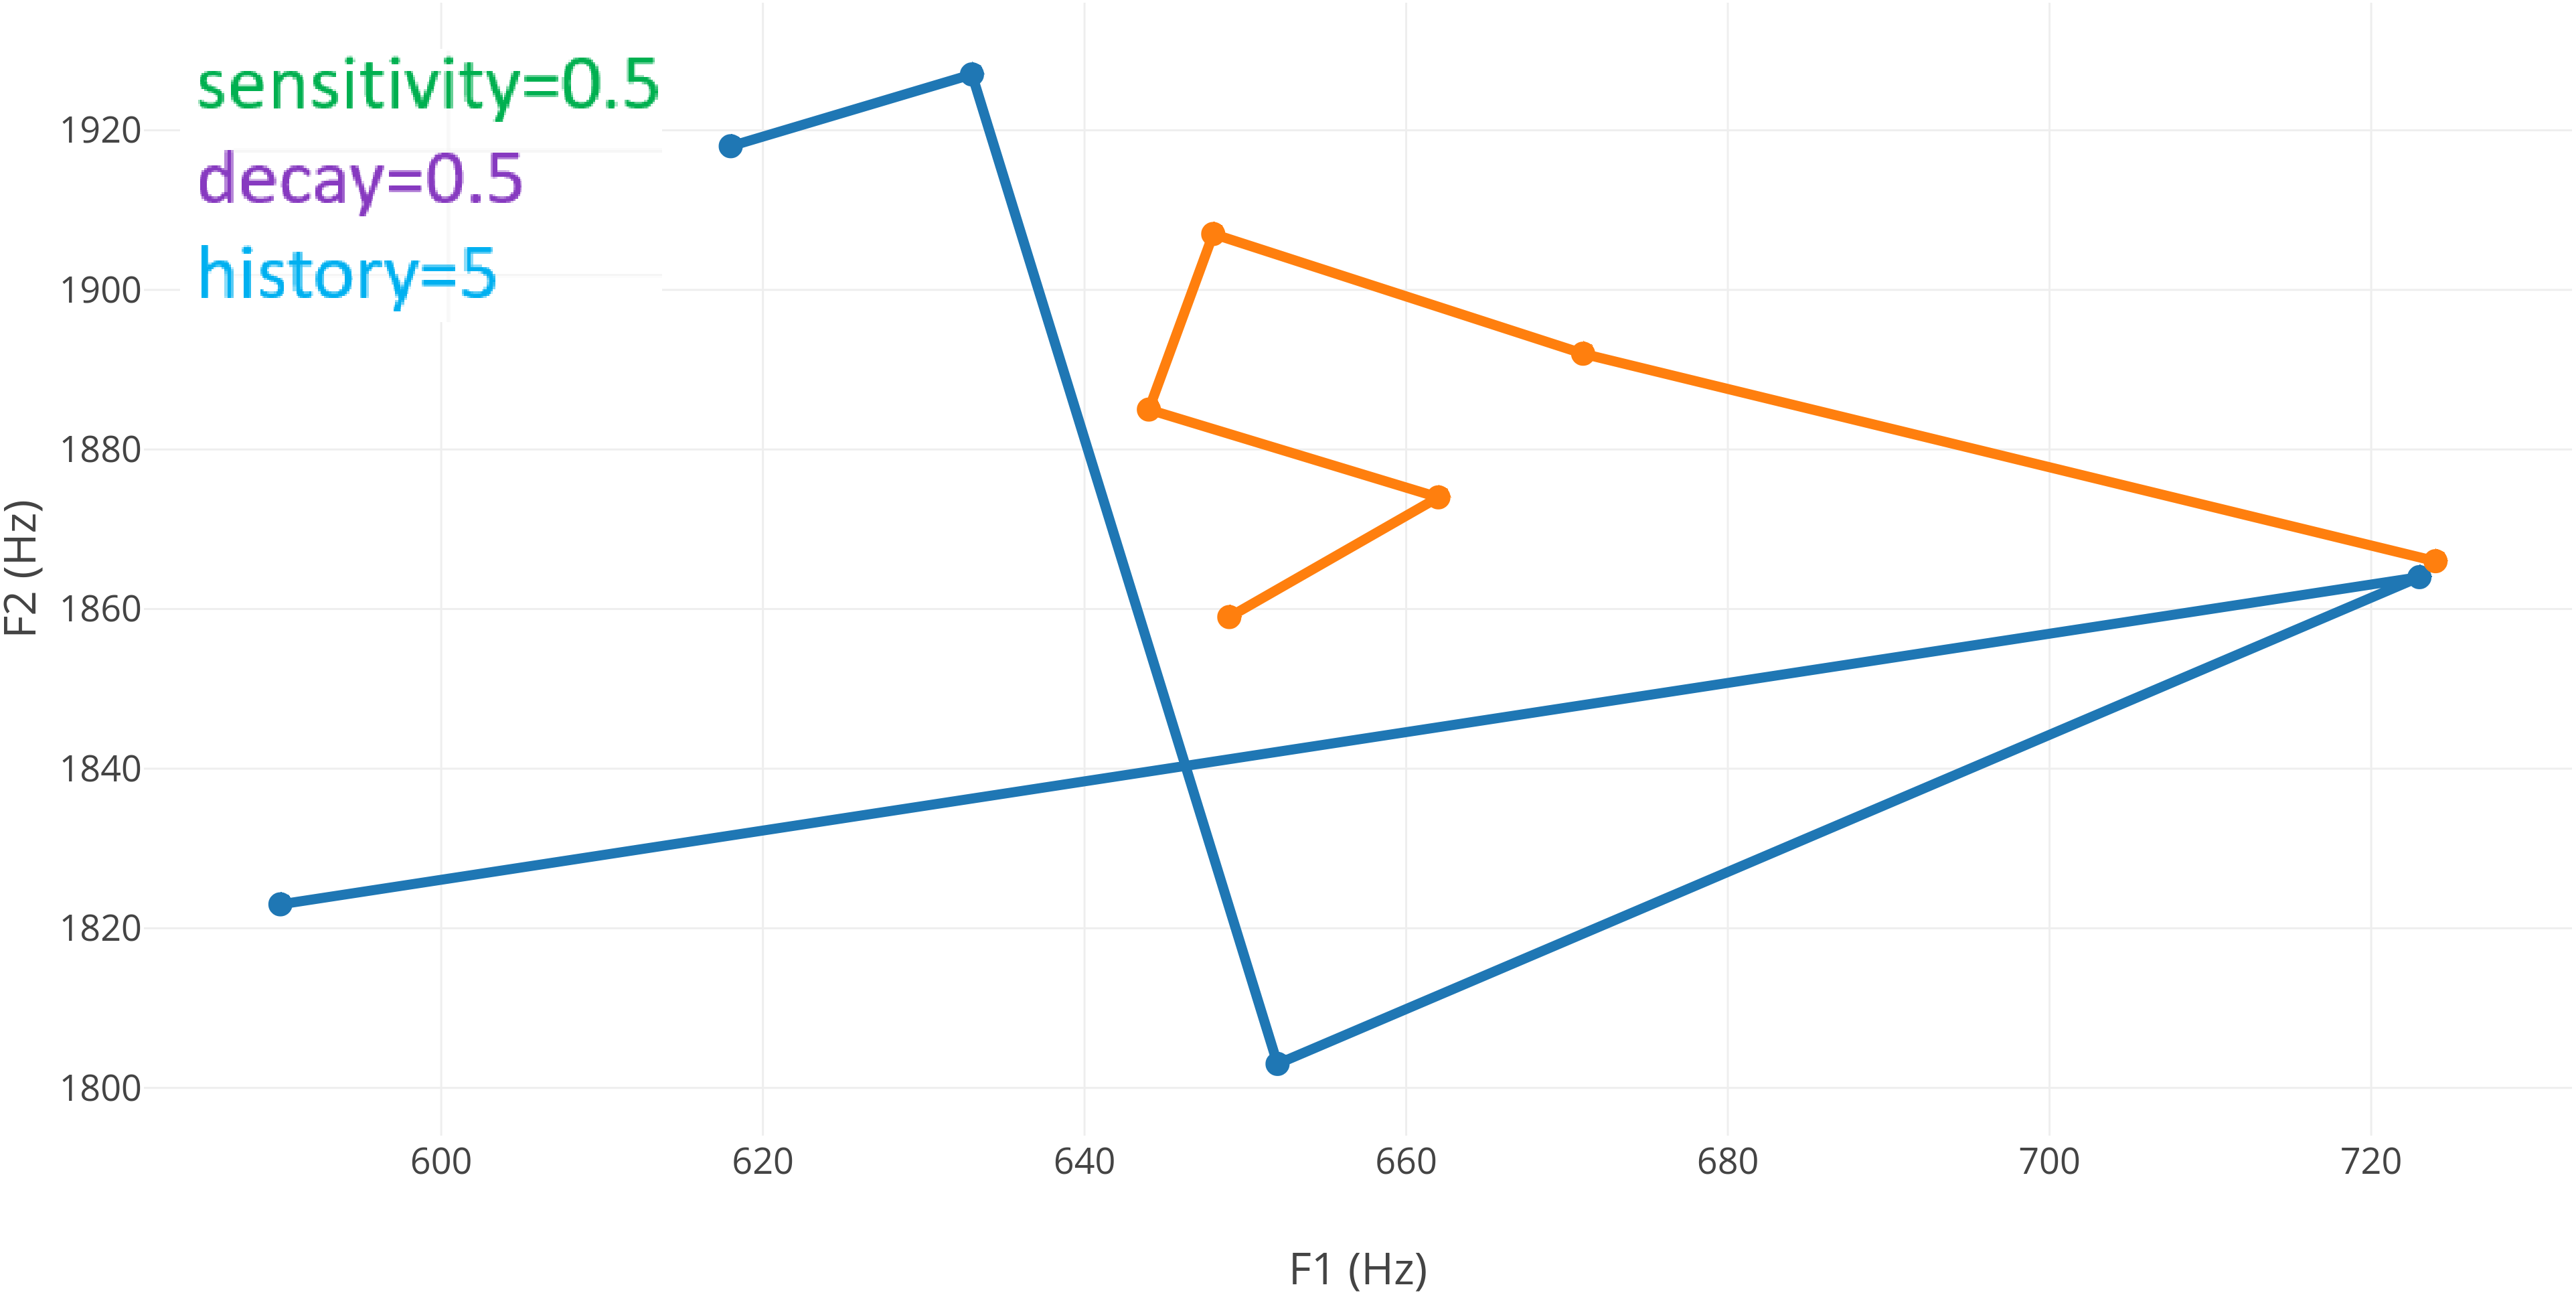
\includegraphics[width=\linewidth]{e_E_05_05_10}
			\end{minipage}
		}
	\end{figure}
\end{landscape}